%!TEX root = ../thesis.tex
%*******************************************************************************
%****************************** Third Chapter **********************************
%*******************************************************************************
\chapter{Outcomes}

% **************************** Define Graphics Path **************************
\ifpdf
    \graphicspath{{Chapter3/Figs/Raster/}{Chapter3/Figs/PDF/}{Chapter3/Figs/}}
\else
    \graphicspath{{Chapter3/Figs/Vector/}{Chapter3/Figures/}}
\fi

\section{Experiments}
list of experiments:
\begin{itemize}
    \item Monte-Carlo rollouts through a 1-dimensional transition function to create a distribution over trajectories.
    \item Monte-Carlo rollouts through a 1-dimensional transition function with uncertainty decomposition and sequentially adding more data.
    \item Trajectory rollouts 
\end{itemize}
\subsection{Environments}

\begin{table}
\caption{Even better looking table using booktabs}
\centering
\label{table:good_table}
\begin{tabular}{l c c c c}
\toprule
\multirow{2}{*}{Dental measurement} & \multicolumn{2}{c}{Species I} & \multicolumn{2}{c}{Species II} \\ 
\cmidrule{2-5}
  & mean & SD  & mean & SD  \\ 
\midrule
I1MD & 6.23 & 0.91 & 5.2  & 0.7  \\

I1LL & 7.48 & 0.56 & 8.7  & 0.71 \\

I2MD & 3.99 & 0.63 & 4.22 & 0.54 \\

I2LL & 6.81 & 0.02 & 6.66 & 0.01 \\

CMD & 13.47 & 0.09 & 10.55 & 0.05 \\

CBL & 11.88 & 0.05 & 13.11 & 0.04\\ 
\bottomrule
\end{tabular}
\end{table}

\subsubsection{Cart-Pole Swing Up}
The cart-pole swing up problem shown in Fig. \ref{Fig:cartpole-environment} is the simplest of the three environments used for experimentation. It consists of a cart of mass $m_1$ and a pendulum of mass $m_2$ and length $l$ that is free to swing about the pivot with which it is connected to the cart. The angle of the pendulum $\theta_2$ is measured anti-clockwise from the downward position. Continuous control actions $u$ applied to the cart cause it to move horizontally in the $x$-direction. The objective of the task is to actuate the cart in such a way that the pendulum is swung to the upright vertical position and balanced there while positioning the cart in the centre of the system at $x=0$.
\begin{figure}[H]
\centering    
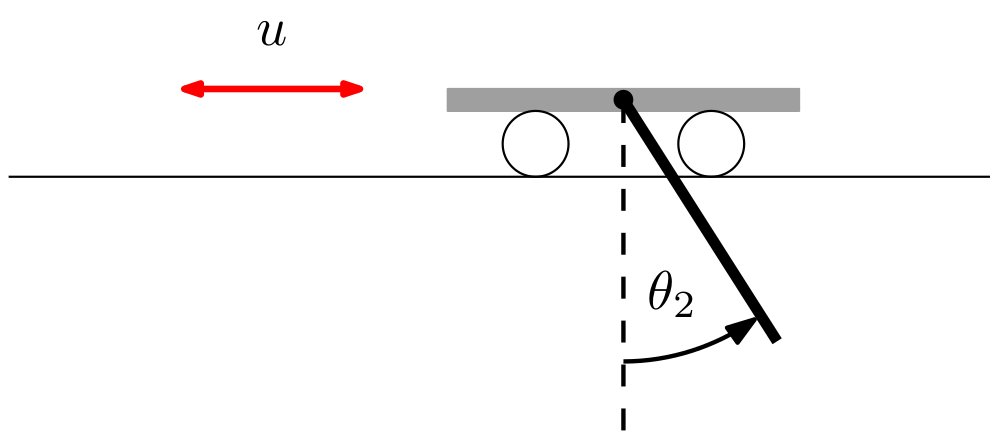
\includegraphics[width=0.5\textwidth]{Chapter3/Figures/cart-pole.png}
\caption[Cart-pole PILCO environment]{Cart-pole swing up. Source \cite{deisenroth2013pilco-documentation}.}
\label{Fig:cartpole-environment}
\end{figure}
The system has 4 continuous state variables: the position of the cart $x$, the velocity of the cart $\dot x$, the the pendulum angle $\theta_2$ and the angular velocity of the pendulum $\dot \theta_2$ of the pendulum. There is a target associated with each state variable.

\subsubsection{Pendubot}
The Pendubot shown in Fig. \ref{Fig:pendubot-environment}  is the second most complex environment used for experimentation. It consists of a central and outer pendulum of masses $m_1$ and $m_2$ and lengths $l_1$ and $l_2$, respectively. The two pendulums are linked together as well as the central pendulum being linked to the ground. The central and outer pendulum angles are given by $\theta_2$ and $\theta_3$, respectively, are measured anticlockwise from the upright vertical position. The link between the ground and the first pendulum can be actuated by the agent by applying a torque $u$ to the joint. The link between the pendulums cannot be actuated making the robot under actuated. The objective of the system is to actuate the central joint in such a way as to swing both pendulums to the upright vertical position and balanced there.
\begin{figure}[H]
\centering    
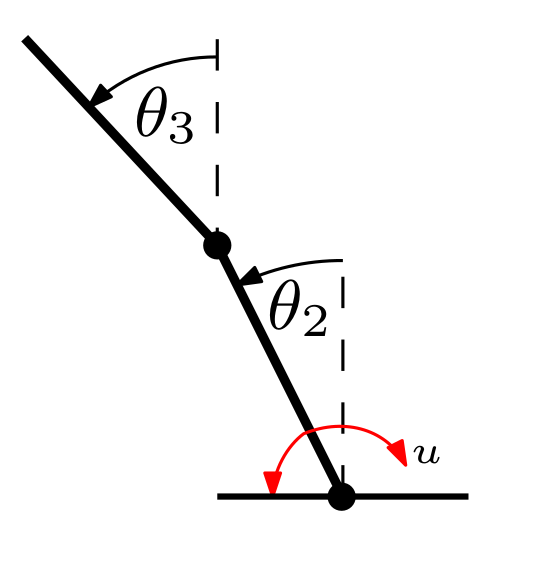
\includegraphics[width=0.25\textwidth]{Chapter3/Figures/pendubot.png}
\caption[Pendubot PILCO environment]{Source \cite{deisenroth2013pilco-documentation}.}
\label{Fig:pendubot-environment}
\end{figure}
The system has 4 continuous state variables: the angles of the pendulums $\theta_2$ and $theta_3$ and the angular velocities of the pendulums $\dot \theta_2$ and $\dot \theta_3$. There is a target associated with each state variable.

\subsubsection{Cart-Double-Pendulum}
The cart-double-pendulum shown in Fig. \ref{Fig:cartDoublePendulum-environment} is the most complex environment used for experimentation. It consists of a cart of mass $m_1$ and a central and outer pendulum of masses $m_2$ and $m_3$ and lengths $l_2$ and $l_3$, respectively. The two pendulums are linked together as well as the central pendulum being linked to the cart.  The central and outer pendulum angles are given by $\theta_2$ and $\theta_3$, respectively, and are measured anticlockwise from the upright vertical position. Continuous control actions $u$ applied to the cart cause it to move horizontally in the $x$-direction. The objective of the task is to actuate the cart in such a way that the double pendulum system is swung to the upright vertical position and balanced there while positioning the cart in the centre of the system at $x=0$. The unconstrained double pendulum system exhibits rich dynamical behaviour and is a chaotic system.
\begin{figure}[H]
\centering    
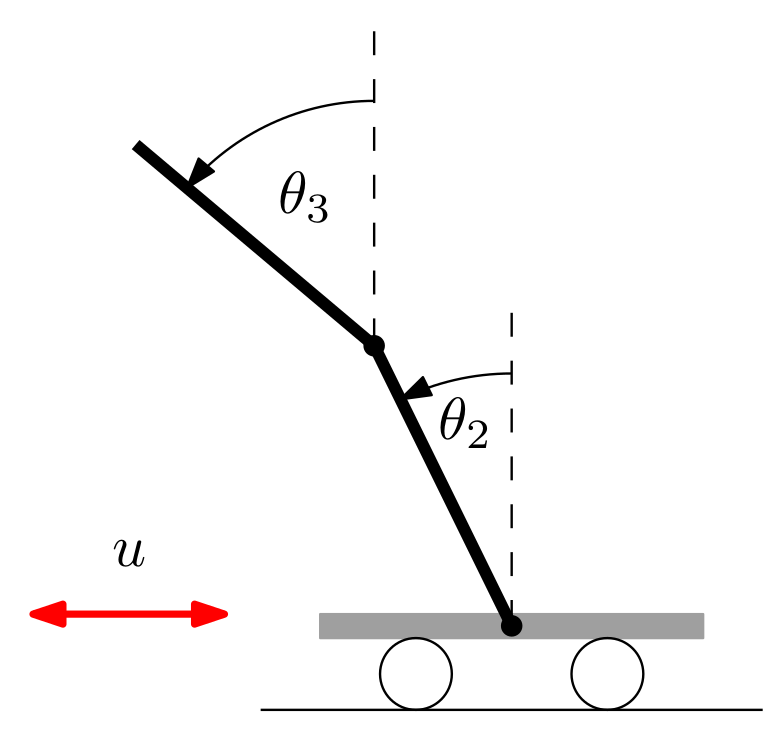
\includegraphics[width=0.3\textwidth]{Chapter3/Figures/cart-double-pendulum.png}
\caption[Cart-double-pendulum PILCO environment]{Source \cite{deisenroth2013pilco-documentation}.}
\label{Fig:cartDoublePendulum-environment}
\end{figure}
The system has 6 continuous state variables: the position of the cart $x$, the velocity of the cart $\dot x$, the angles of the pendulums $\theta_2$ and $theta_3$ the angular velocities of the pendulums $\dot \theta_2$ and $\dot \theta_3$. There is a target associated with each state variable.



\section{Results}
RESULTS THAT I HAVE
\begin{itemize}
    \item Cartpole
\end{itemize}

A list of plots that I want:

\begin{itemize}
    \item Plots of number of basis functions for each environment used and maybe also convergence plots.
    \item Plot of a 1D transition function showing the distribution over trajectories on the side. Perhaps also a distribution over losses. I have the GP notebook to do this already.
    \item Plot showing 1D function with uncertainty breakdown and how it decreases with more data as we become more confident about the weights.
    \item For each environment, plot of the actual trajectories for the solved environment and a plot of the MC trajectories for the solved environment.
    \item Plots showing that when PILCO is not learning it is choosing policies with high reward but low epistemic uncertainty.
    \begin{itemize}
        \item How to achieve this: 
    \end{itemize}    
\end{itemize}

\section{Discussion}

\section{Conclusion}



